\minitoc


In the context of the Internet of Things, as defined in Section \ref{S_assumptions}, a framework for zero-fee transactions in the Internet of Things (\hyperref[obj:1]{\emph{Objective 1}}) should consider transactions to be granted access to physical devices
, e.g., cars and doors, but also to the data generated by the devices, as those data are valuable.
To this end, we will focus in this chapter on designing a framework that:

\begin{itemize}
  \item provides access control on physical devices and goods; 
  \item provides access and usage control on data; 
  \item has no fee, or very low fees, to enable micro-transactions;
  \item preserves the privacy of both participants of a transaction;
  \item considers the performance and the security requirements of the Internet of Things.
\end{itemize}

This chapter is structured as follows. First, the IOTA technology, a distributed ledger with zero-fee transactions is introduced in Section \ref{S_iota_dlt}. IOTA uses a DAG to build its transaction graph 
(cf. Section \ref{ss_blockchain_DLT}), and was designed to answer the performance requirements of the Internet of Things. IOTA is the key technology of the 
framework, from which the other tools are derived. Then, the framework and its components are detailed in Section \ref{S_framework}. Finally, a security and privacy threat assessment is conducted in Section \ref{S_security_and_privacy_evaluation}.
A conclusion of the chapter is provided in Section \ref{S_conclusion_ifip}.

\section{IOTA distributed ledger}
\label{S_iota_dlt}
In this section, we introduce IOTA as a key technology of the proposed framework, since most of the tools presented 
are derived or adapted to this distributed ledger.
As discussed in Section \ref{S_DLT_performance}, blockchain technology has several security and performance drawbacks 
for the Internet of Things which limits its 
adoption. Besides, transaction fees in some public blockchains can 
be greater than the actual transaction value, making micro-transactions impossible. Removing transaction fees in blockchains 
is an intricate issue since transaction
fees are used as an incentive for creators of blocks to contribute to the network. These different issues justify the need 
to introduce a new paradigm for 
cryptocurrency transactions. 

\subsection{\rul{Identifying DAG-based distributed ledgers for Internet of Things performance}}

 \rul{As part of the second research objective} (\hyperref[obj:23]{\emph{Objective 2}}), \rul{it is necessary to identify the most suitable distributed ledger technology for the Internet of Things. Distributed ledger technologies are interesting in the first place, due to the partial decentralization they provide and due to the immutability of the ledger which is useful for several applications, e.g., trust management, secure and private transactions (cf. Section} \ref{ss_motivation}). 

 \rul{In the state of the art} (Chapter \ref{C_state_of_the_art}), \rul{we introduced different criteria to differentiate distributed ledgers: consensus methods, performance metrics or the nature of the transaction ledger. In particular, distributed ledgers based on a directed acyclic graph or the Hashgraph have very attractive metrics. In theory, they both provide high throughput, i.e., numerous transactions per second, which is not often the case for blockchain-based distributed ledgers.}

 \rul{Yet, directed acyclic graphs are a better alternative as:}

 \begin{enumerate}
   \item DAGs are permissionless ledgers\footnote{It is although possible to deploy private instances of directed acyclic graphs, cf. Section \ref{ss_testbed}} in contrast to Hashgraph, and provide a higher degree of decentralization;
   \item Hashgraph is a project poorly studied by academia while DAGs, in particular IOTA, are being increasingly studied by the research community;
   \item the bandwidth requirements of Hedera's Hashgraph set a high barrier to entry for nodes, limiting its adoption for the Internet of Things. Nodes require at least 256 GB of RAM and 24-core or better CPU hyperthreaded (48 threads) as a minimum.
 \end{enumerate}

\rul{If distributed ledgers using a directed acyclic graph for their transaction ledger are suitable for the Internet of Things, the choice of IOTA rather than other DAG technologies, e.g., Obyte or Nano, is further motivated in Section} \ref{ss_benefits_iota}.

\subsection{A DAG-based transaction ledger}
IOTA builds its transaction graph using a directed acyclic graph (cf. Section \ref{ss_blockchain_DLT}) called the \emph{Tangle}. The difference between the tangle and a blockchain is represented in Figure \ref{F_dag_vs_blockchain}.
IOTA has properties common to DAG-based distributed ledgers, i.e., low transaction fees, disintermediation, and high throughput.
As a reminder of Section \ref{ss_blockchain_DLT}, transactions in a network based on a directed acyclic graph are built as follows. 
The transactions are the vertices of the transaction graph. There is only one transaction by vertice.
When a new transaction arrives, it must approve two previous transactions. The approval is materialized by an edge. These
approvals are represented by directed edges. If there are no
directed edges between two transactions $A$ and $B$, but there is a directed
path of length at least two from $A$ to $B$, we say that $A$ indirectly approves $B$.
There is an original transaction, which is approved directly or indirectly by all the transactions, called \emph{the Genesis transaction} 
in IOTA. 

The genesis is described in the following way. At
the beginning of the tangle, there was a single address with a balance that contained all
IOTA tokens. The Genesis transaction sent these tokens to several other addresses belonging to the founders. All of the tokens were created in the genesis transaction and as there is no mining, it is impossible 
to create iota tokens without \emph{taint}.
A token is considered tainted if it belongs to at least one identifying address on the IOTA ledger. 
Only iotas that have never been linked to any identifiable address, i.e. an address belonging to someone who has been re-identified, can be considered as untainted~\cite{Tennant2017}.

Finally, for a transaction site on the IOTA ledger, there is an associated \emph{weight} $w$. The general idea behind this notion is that 
a transaction with a significant weight is more important and trusted. Along weight, the notion of \emph{cumulative weight} $w_{cum}$ of a transaction $t$
 is also introduced, as the sum of its weight plus the weight of all transactions validating (including indirectly)  the transaction $t$.
 In Figure \ref{F_dag_vs_blockchain}, both weights and cumulative weights (respectively $w$ and $w_{cum}$) are given inside the sites of the DAG.
 For instance, the transaction $F$ has a weight $w_F = 2 $, is directly validated by $B$ and $E$ and indirectly by $A,C,$ and $D$. 
 Therefore, the cumulative weight of $F$ is $w_{cum,F}= (w_A + w_B + w_C + w_D + w_E) + w_F = 1+1+1+1+4+2 = 10$.  
\begin{figure*}[t]
\centering
 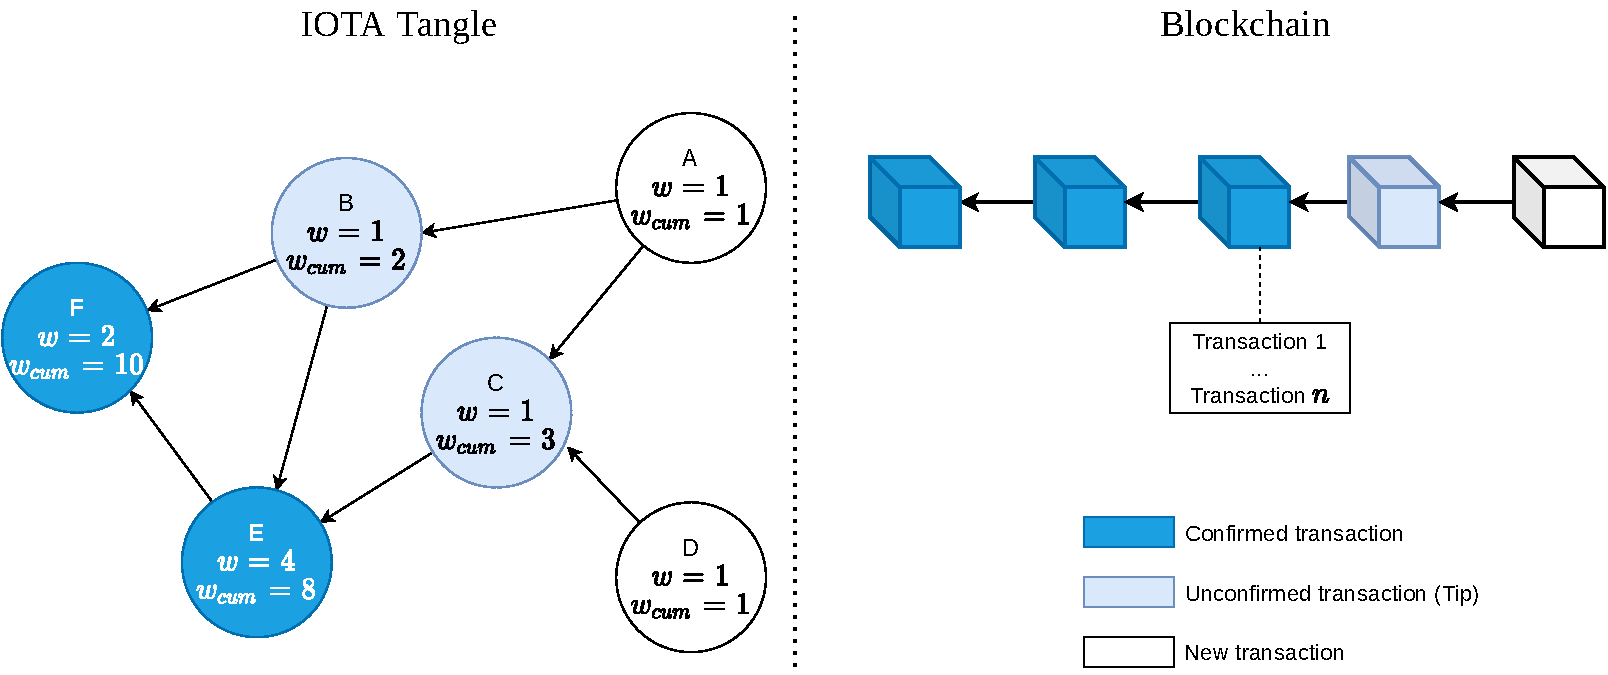
\includegraphics[width=\textwidth]{Images/IOTA_vs_blockchain.pdf}
\caption{Transaction ledger in the Tangle (directed acyclic graph) and a blockchain. Each transaction site on the DAG has a weight $w$ and an indirect 
cumulative weight $w_{cum}$}
\label{F_dag_vs_blockchain}
\end{figure*}

\subsection{Consensus method}
\label{ss_consensus_method}

In IOTA, to issue a transaction, users must
work to approve other transactions, so that users themselves are
contributing to the network’s security. The nodes check in particular if the
approved transactions are not conflicting. If a node finds a transaction conflicting with the tangle history, the node will not approve the conflicting transaction
directly or indirectly. In case a node issues a new transaction that validates conflicting transactions, it is at risk that other
IOTA nodes do not approve its transaction. As a transaction receives additional approvals, i.e., its weight is increasing, it 
gets a higher level of confidence. It consequently becomes harder for the system
to accept double-spending transactions.

A new transaction, i.e., not approved by other transactions, in the IOTA network, is called a \emph{tip}. To issue a new transaction, an IOTA node proceeds to the following steps:

\begin{itemize}
  \item The node picks two other transactions to approve according to a \emph{tip selection algorithm} (TSA);
  \item The node checks if the two transactions are conflicting;
  \item The node solves a cryptographic challenge to prevent spam. It works exactly like Bitcoin's proof of work, 
  but the challenge is not designed to pick the next miner, but only to make sure a node can not spam the network 
  by pushing too many transactions simultaneously.
\end{itemize}

The IOTA network is asynchronous, which means that the tangle may contain conflicting transactions. However, the nodes \emph{do not 
have to achieve consensus} on which transactions are valid and should be in the tangle, which is a significant difference with blockchains. 
That implies that all the transactions can be in the ledger. However, if there are two conflicting transactions, the nodes 
have to decide which transaction will be \emph{orphaned}, i.e., not validated indirectly by new transactions.

\textbf{Tip selection algorithm.}
In IOTA, the tip selection algorithm (TSA) determines which tips should be approved and referenced in new transactions.
 It aims to achieve a balance between security and network efficiency.
The tip selection algorithm in IOTA is based on a \emph{Monte Carlo Markov Chain} (MCMC).
The MCMC algorithm takes into account various factors such as the cumulative weight of transactions, 
the transaction arrival rate, and the network topology. By considering these factors,
 the algorithm selects tips that are more likely to be included by other transactions in the Tangle, 
 increasing the chances of approval for the users and overall transaction confirmation.
The tip selection algorithm plays a crucial role in the security and performance of the IOTA network. It helps prevent the concentration of approvals on a single branch of the Tangle,
 improving the resilience against potential attacks. 
Additionally, the algorithm aims to maintain a balanced distribution of transaction approvals across the network,
 ensuring efficient propagation and confirmation of transactions.

 \subsection{Benefits of IOTA}
\label{ss_benefits_iota}
 IOTA is a DAG-based distributed ledger and therefore has the attractive features of this technology. These benefits have been listed in Section \ref{ss_blockchain_DLT} and are the following:

 \begin{itemize}
  \item writing transaction is not energy-intensive, enabling low-power devices to participate in the network;
  \item throughput is high after the bootstrapping stage and increases with the number of users;
  \item users add their transactions directly to the network without relying on any intermediaries, such as miners or gateways.
\end{itemize}

In particular, the high throughput answers the scalability requirements of large-scale networks (cf. Section \ref{S_assumptions}) as it enables to process the high volume of transactions. In addition, IOTA does not have any transaction fee due to the removal of miners (\hyperref[obj:1]{\emph{Objective 1}}), while other distributed ledgers using a DAG have small fees \cite{Churyumov2017, LeMahieu2017}. IOTA is also largely studied and used in the literature \cite{Alshaikhli2022, Conti2022, Guo2023, Alsadi2023}, and the IOTA foundation, the main actor supporting the development of IOTA, also contributes to the scientific literature\footnote{https://www.iota.org/foundation/research-papers}. Finally, IOTA is built to be resistant to an adversary with a quantum computer \cite{Popov2017}, which is an interesting property from long-term security that distinguishes IOTA from its competitors.


\subsection{Limits of IOTA}
\textbf{Reliance on the Coordinator.} The IOTA network, in its current version (1.0, June 2023), relies on an entity called \emph{the coordinator}.
The coordinator is a centralized component that was initially introduced to ensure the security of the network during the bootstrapping phase.
The coordinator's purpose is to issue \emph{milestones} that validate transactions and to help prevent certain types of attacks, notably the double-spending attack.
Even though the coordinator is a temporary device that is supposed to be removed in the IOTA 2.0 \cite{Popov2020}, it is still currently used 
and creates the following issues:
\begin{itemize}
  \item \emph{Centralization}: The coordinator gives a single entity control over the network's security, making it a point of failure and potential vulnerability.
  Indeed, if the coordinator is stopped or under a denial of service attack, the transactions can not be validated anymore;
  \item \emph{Trust}: the coordinator is run by the IOTA Foundation, which should be trusted by the participants. It 
  goes against the trustless and transparent nature of blockchain networks;
  \item \emph{Timeline}: the timeline for the removal of the coordinator has not been set yet, and 
  the network has been running since 11 July 2016.  
\end{itemize}


\textbf{Scalability issues.} IOTA distinguishes (in version 1.0) two different regime types, based on the number of 
simultaneous tips in the network \cite{Popov2017}. The \emph{low load regime}  has a small number of tips, typically one tip.
The flow of transactions is so small that it is unlikely that two different transactions approve the same tip. The 
low load regime is characterized by a low latency. Conversely, the \emph{high load regime} has a large number of tips. 
The flow of transactions is large, and both computational delays, as well as higher network latency, increase the likeliness of 
two simultaneous transactions approving the same tip. 


\subsection{IOTA 2.0 and the Coordicide}
The removal of the coordinator is a process called \emph{the coordicide} \cite{Popov2020} that is due to thoroughly change the 
IOTA network mechanisms. We provide an overview of the anticipated changes in IOTA 2.0, the post-coordicide version of IOTA.

  \textbf{Node accountability.} In a network where the coordinator has been removed, several applications require to
  associate transactions and messages with the node which issued them. This is true for the rate control mechanism and the 
  voting-based consensus detailed next. To make the node accountable, IOTA 2.0 requires the introduction of a \emph{global node identity}.
 Node identities are achieved using common public key cryptography to sign data and link it to the issuing node.
  The issuing node adds its public key to every signed message so that every node can verify its authenticity.

  The introduction of node identities is troublesome as it exposes IOTA to \emph{sybil attacks}, in which
  attackers create multiple fake identities to get a disproportionate weight in the network. To solve this issue, 
  IOTA 2.0 relies on \emph{mana}, which is obtained when a node issues transactions. Mana is the basis of a 
  reputation system, to identify the reliable nodes which contribute the most to the network.

  \textbf{Rate control mechanism.} In an overload scenario, where the nodes 
  are trying to issue more transactions than the overall network can handle, e.g., due to its
  physical limits, particular transactions originating from the most heavily
  contributing nodes should be either limited or penalized. It is achieved in IOTA 2.0 
  by using an \emph{adaptive proof of work}. The adaptive proof of work is determined thanks to 
  three parameters: the base difficulty, an adaptation rate that depends on the mana owned by the node, 
  and finally, a time window that defines the granularity of the rate control mechanism. The shorter the time window, 
  the quicker the network reaction is when the node issues too many transactions.

  \textbf{Consensus and voting.} In IOTA 1.0, the consensus is achieved 
  by applying the tip selection algorithm, i.e., the mechanism used by
  nodes to select the transactions to approve, based on a biased random walk.
  IOTA 2.0 is based on a new consensus method, called \emph{Shimmer}.
  The idea behind this new consensus mechanism is to care only about the knowledge of a very small subset of
  nodes, instead of the opinion of every other node. The actual consensus method used by IOTA 2.0 is called 
  \emph{Fast probabilistic consensus} \cite{Cooper2015, MallmannTrenn2017}, and relies on the idea
  that randomized voting, i.e., random queries, are sufficient for
  good performance, and due to the small message complexity, makes the protocol scalable.
  Another advantage of this randomness is the improved robustness in less reliable networks and situations 
  with dynamicity, where nodes join and leave the network frequently.

\section{A framework for performance, security and privacy in the Internet of Things}
\label{S_framework}
To answer the performance, privacy and security needs of the Internet of Things, and to enable zero-fee transactions (\hyperref[obj:1]{\emph{Objective 1}}),
the following framework is proposed. It is designed to address the different needs simultaneously, as well as to cover the different 
categories of Internet of Things use cases, by considering both data and physical accesses. The different components are detailed next, after a general overview.

 \subsection{Framework overview}

 \rul{As IOTA has been identified as a suitable technology to address Internet of Things requirements (as part of this chapter's contribution), the proposed framework will be based on IOTA and auxiliary existing technologies.}
 
 The proposed framework is made up of the following components (cf.~Figure~\ref{F_framework_IFIP}):

\begin{enumerate}
\item IOTA technology, as a suitable distributed ledger technology to answer IoT performance requirements and its zero-fee transactions;
\item IOTA Access, an open-source framework used to control access to IoT devices. It is developed by the IOTA Foundation to complement the IOTA technology; 
\item a Usage Control System, to monitor the usage and dissemination of the data in the system. The UCS relies on a Trusted Environment Execution of the device of the monitored user;
\item a decentralized mixing service coupled with merge avoidance (cf. Section \ref{ss_obfuscation_coin_mixing_merge_avoidance}), to obfuscate the transactions and improve the privacy of users \cite{Sarfraz2019}.
\end{enumerate}
 \begin{figure*}[t]
    \centering
     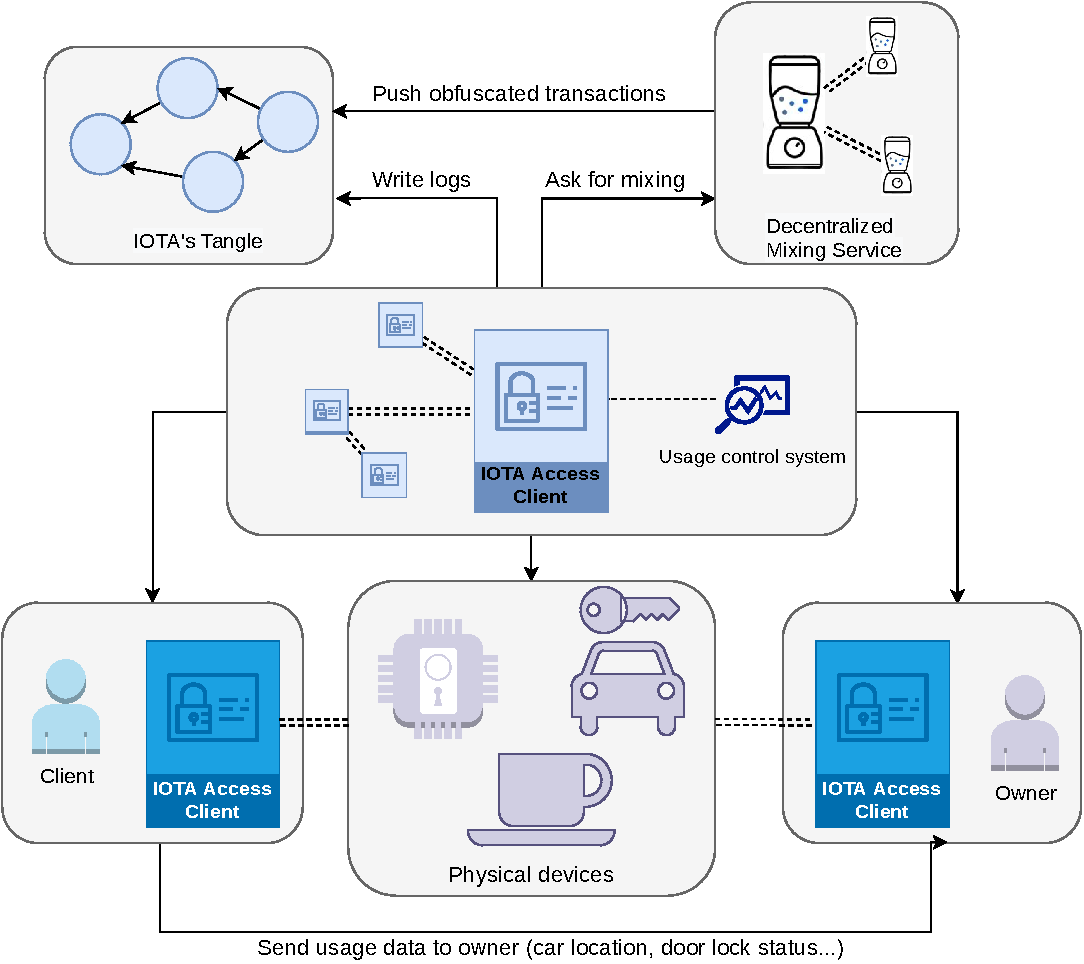
\includegraphics[width=0.75\textwidth]{Images/framework_IFIP.pdf}
    \caption{Framework to monitor data usage and physical access to IoT devices based on privacy-preserving transactions}
    \label{F_framework_IFIP}
    \end{figure*}
  
  \rul{IOTA and IOTA Access have been developed and maintained by the IOTA foundation and the mixing scheme has been proposed by Sarfraz \emph{et .al}} \cite{Sarfraz2019}.  
  IOTA and usage control have been already described in previous sections (respectively, Section \ref{S_iota_dlt} and Section \ref{S_usage_control}). In the following, 
  we detail the two other components of the framework, IOTA Access and the decentralized mixing service for IOTA.  
 \subsection{IOTA Access}
 
 IOTA Access is a lightweight access control framework tailored for resource-constrained networks.
 It is based on XAIN's FROST project, which is the byproduct of Leif-Nissen Lundbaek's Ph.D. Thesis at Imperial College London \cite{Lundbaek2020}.
 The framework is also expanded with relevant concepts, such as obligations and the delegation of access-control policies,
  to particularly address the need for reliable and secure human-machine interactions in the IoT. Notably, IOTA Access 
  introduces the concept of \emph{actions}, which are all the authorized actions that a user can perform. Actions 
  are based on \emph{attributes, obligations} and \emph{conditions}, very similar to the UCON notions with the same terminology (cf. Section \ref{S_usage_control}), but used
  in the context of physical access instead of data access. In particular, empowered by obligations and conditions, it is possible with IOTA Access to:
     1) grant or deny access at any time;
    2) charge users for physical access with zero-fee transactions; 3) set complex access restrictions based on conditions and obligations.
    To do so, IOTA Access is divided into three components, represented in Figure \ref{F_iota_access}:

    \begin{itemize}
      \item the \emph{IOTA Access client}, which is a mobile access client used as the user interface,
       both for creating policies and initiating access requests. IOTA Access contains an Android-based reference implementation;
       \item the \emph{IOTA Access server}, the embedded software executed on the device for which access will be delegated;
       \item the \emph{IOTA Access policy store}. It consists of interface servers for managing policies;
    \end{itemize}
  

 \begin{figure*}[t]
   \centering
    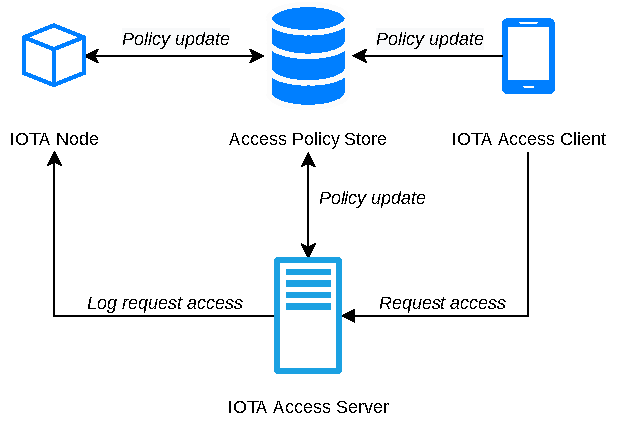
\includegraphics[width=0.6\textwidth]{Images/iota_access.pdf}
   \caption{IOTA Access framework representation}
   \label{F_iota_access}
   \end{figure*}

 The interactions between the IOTA Access components are as follows, also represented in Figure \ref{F_iota_access}. Users deploying an IOTA Access client can either request access to devices or update access policies enforced on their own devices.
 In the first case, if a user requires access to a device, the IOTA Access server evaluates the request against the policy, then logs the 
 request on the IOTA ledger, possibly using a private Tangle rather than the public ledger. In the second case, a user-triggered policy update causes a chain of network exchanges between the IOTA Access components.
First, the IOTA Access clients directly update the policies in the IOTA Access policy store, which forwards the update to the IOTA Access server and notifies the IOTA node of the update for logging purposes. 

IOTA Access is used in the proposed framework to extend the zero-fee privacy-preserving transactions to the Internet of Things devices, 
instead of restricting them to data-sharing use cases.
 \subsection{Decentralized mixing for IOTA.}
 \label{ss_decentralized_mixing_iota}
Coin mixing has been introduced in Section \ref{ss_obfuscation_coin_mixing_merge_avoidance} as one of the most common tools to obfuscate transactions 
in distributed ledgers. Coin mixing aims at removing the link between the sender and the receiver of a transaction, to complicate re-identification attacks.
However, centralized coin mixing creates significant security and privacy risks. The centralized mixing service is a likely target for denial of service 
attacks and may steal the funds or keep the transaction records for itself (cf. Section \ref{ss_obfuscation_coin_mixing_merge_avoidance}). 
However, decentralization is troublesome due to the possibility to conduct edge insertion attacks. While this is true for most public blockchains, which require transaction fees, it is 
different for IOTA due to its transaction mechanisms.

Indeed, Sarfraz \emph{et al.} \cite{Sarfraz2019} designed a decentralized mixing scheme for IOTA that leverages zero-fee transactions 
and does not require changes in the IOTA protocol. The mixing scheme has the following attractive features:
\begin{itemize}
  \item protection against signature forgery and the guarantee that
  even in the presence of malicious adversaries during mixing,
  no participant can reveal portions of his/her private key of the
  input address. This property is guaranteed by \emph{multi-signatures};
  \item fully decentralized mixing operation;
  \item no mixing fees from participant;
  \item anonymity, availability and correctness are guaranteed (cf. Section \ref{ss_obfuscation_coin_mixing_merge_avoidance});
\end{itemize}

\textbf{Mixing preliminaries.} \rul{We now introduce further considerations on IOTA addresses and mixing for a better understanding of the mixing protocol which will be detailed next. An IOTA \emph{transaction} is a transfer of IOTA tokens between a set of IOTA
addresses. To issue a transaction, a user
specifies one or more input addresses $A_{1},..., A_{n}$ with a
positive value $z$ and output (receiving) addresses $A_{1},..., A_{n}$. IOTA also supports \emph{zero value} transactions, without any input addresses. In order to
spend from an input address, a user needs to
sign the transaction with the corresponding private key to prove it owns the input address. 
}

\rul{\emph{IOTA addresses} are defined using a ternary numeral system and have a length of 81 trytes. A private key is associated with each address, whose size is determined according to a security level $s$. Once the private key is generated, it is hashed into 27 fragments that are each hashed 26 times. The hashed key fragments are used to generate an address. }

\rul{A \emph{multi-signature scheme} is a digital signature scheme that allows a group of users rather than a single one
to sign a document. A multi-signature, in cryptocurrencies, enables a group of people to formally agree on spending. Ideally, all participants need to sign the transaction from a multi-signature address, but certain variations in the
multi-signature scheme $(m, n)$ allow ownership to a given number of participants. A $(m, n)$-threshold signature scheme is a digital signature scheme where any $m$ or more signers from a group of $n$ signers can produce signatures on behalf of the whole group. In order to create a multi-signature address all participants need to share their \emph{digests} publicly, which are then concatenated to make a long single
digest. Then the same process is followed
to create a multi-signature address of 81 trytes.}

\textbf{Mixing protocol design.} We now detail the actual decentralized mixing protocol. It is composed of three different phases: \emph{settlement} (1), then \emph{output shuffling} (2) 
and finally the \emph{transaction} (3) \cite{Sarfraz2019}, all represented in Figure \ref{F_mixing_iota}. In case the protocol can not be completed, another additional \emph{fallback} phase is introduced. The protocol is detailed with $n$ peers, but to achieve anonymity, the protocol requires at least two participants. The first \emph{settlement} phase (1) \rul{using a} ($1, n$) \rul{multi-signature scheme} unfolds as follows :

\begin{enumerate}
  \item[(1a)] each peer $i \in \{1,..., n\} | k_{i},... k_{n} \in {0,1,2,... } $ determines key indexes $k_{1},..., k_{n}$
  and security levels $ s_{1},..., s_{n}$ | $s _{i},..., s_{n} \in {1, 2, 3}$. s is a security level that results in a 
  key of length $ l = s * 27 * 81$ trytes. $k_{i}$ and $s_{i}$ are used to generate digests $d_{i}$ for $i \in {1,..., n}
  $ and private keys $ pr_{1},..., pr_{n}$;
  \item[(1b)] each peer shares the digests $d_{1},..., d_{n}$ to generate $M_{1},...,M_{n}$ multi-signature addresses such that the addresses-digests mapping $M$ is
  \begin{center}
    $M = \left\{\begin{array}{l}M_1 \rightarrow D_{i(1)}, \ldots, D_{n(1)} \\ M_2 \rightarrow D_{i(2)}, \ldots, D_{n(2)} \\ \ldots \\ M_n \rightarrow D_{i(n)}, \ldots, D_{n(n)}\end{array}\right\}$
  \end{center}
  \item[(1c)] for each generated multi-signature address, every $n - i$ peers share their private keys $pr_{1}, pr_{2},..., pr_{n}$ to make a ($1,n$) 
   mapping for address ownership;
   \item[(1d)] Each peer makes a transaction $T_{i}$ to the multi-signature address $M_{i}$;
\end{enumerate}

Mixing peers validate the multi-signature address by sharing digests. If the address validation fails, then a malicious participant may be 
involved in the settlement process. The protocol aborts and all participants receive a notification. The settlement phase is followed by 
the output shuffling phase. The output shuffling phase aims to randomize the set of output addresses declared by the peers, 
preventing peers from mapping input addresses to output addresses. \emph{Shuffling} (2) unfolds as follows:

\begin{enumerate}
  \item[(2a)] each peer creates an IOTA output address $O_{1},...,O_{n}$ corresponding to input addresses $A_{1},..., A_{n}$;  
  \item[(2b)] each participant generates a key pair $(E_{i},D_{i})$ and broadcasts its public key:
  \item[(2c)] once all keys have been broadcast, the first peer creates a layered encryption of its output address, which means 
  that it encrypts its output address with all the keys of the other peers. The first peer then forwards the ciphertext to the next participant;
  \item[(2d)] each following participant $i$ up to the last one $n$ decrypts the outermost layer of encryption for all ciphertexts 
  with its corresponding decryption key $D_{i}$. Each peer receives a list of ciphertexts of size $i -1$ ;
  \item[(2e)] after decrypting the outermost layer of all the ciphertexts, each participant $i$ randomly shuffles the ciphertexts 
  and then creates a nested encryption for its output address $O_{i}$;
  \item[(2f)] the last participant decrypts all the ciphertexts and
 shuffles the final decrypted list with its output address. Finally, the final list of output addresses is forwarded to 
 the other participants.
\end{enumerate}

Upon receiving the decrypted list, the participants check if
their output addresses are actually in the list. If there is a duplication of output addresses 
or if any output address is missing from
the list, the protocol interrupts and peers enter the fallback phase. Additionally, if the decryption fails or multiple decryptions
lead to the same output, the corresponding participant aborts the
protocol and notifies every participant and all the
participants enter the fallback phase as well. If the shuffling phase unfolded correctly, the peers can enter the last transaction phase.

The purpose of the transaction phase is to build and push the final transaction to the network, i.e., the iotas from each input address $A_{1},..., A_{n}$ 
will be transferred to each corresponding output address $O_{1},...,O_{n}$. As input addresses are multi-signature, it is required 
that all the participants sign each transaction. The \emph{transaction} phase (3) is made up of the next steps:
\begin{itemize}
  \item[(3a)] every participant creates a mixing transaction that spends IOTA tokens from each
  of the input addresses in $(A_{1},...,A_{n})$ to $( O_{1},...,O_{n})$.
  \item[(3b)] the participant $i$ signs the transaction according to the specification of the IOTA protocol and broadcasts the signature $S_{i}$;
  \item[(3c)] when it receives a valid signature $S_{j}$ from another peer $j$, the peer $i$ adds all the signatures in the bundle.
 Participant $i$ checks if any other participant has spent their money saved for mixing. 
 If a participant spent its funds, the protocol is aborted and the fallback phase is triggered;
 \item[(3d)] the participant $i$ receives two transactions to approve as part of the IOTA transactional protocol (cf. Section \ref{S_iota_dlt}),
 performs the proof of work to prevent spamming, then generates the transaction hash 
 and broadcast the bundle ($S_{1},...,S_{n}$) to the IOTA network.
\end{itemize} 

If the transaction phase is completed, the mixing process is achieved and the mixing desired properties, i.e., anonymity, availability and correctness, are provided.
However, at any step of the mixing process, the protocol can enter the fallback phase in case of misbehavior. 
The protocol needs to be run again with new unused output addresses for correct protocol execution. 
The full protocol with a correct execution, i.e., excluding the fallback phase, 
is represented in Figure \ref{F_mixing_iota} \rul{with three honest participants}.

\rul{The first \emph{settlement} phase (1) unfolds as follows.  Alice, Bob and Charlie generate the multi-signature addresses $M_1, M_2$ and $M_3$ and share their corresponding private keys. The three participants then make the transactions $T_1, T_2$ and $T_3$ to the generated $M_1, M_2$ and $M_3$ addresses respectively (step 1d).
After the settlement starts the \emph{shuffling} phase (2).
In step (2a), the participants Alice, Bob and Charlie generate output addresses $O_{1}, O_{2}$ and $O_{3}$ respectively. In the next step (2b),
each participant except for Alice creates an encryption and decryption key pair. Bob and Charlie broadcast their encryption keys
$E_{k}B$ and $E{k}C$. In the following step (2c), Alice sequentially encrypts her output address $O_{1}$ i.e., Alice first encrypts for Charlie obtaining $c_1 = E(E_{k}C, O_1 )$ and then for Bob obtaining $c2 = E (E_{k}B, c_1 )$. Alice finally adds $c_2$ to a list $L = (c_2)$ and forwards $L$ to Bob. In steps (2e) and (2f), Bob receives $L$
from Alice, then decrypts the outermost layer of the cipher text $c_2$ in the list
$L$, obtaining $c_1$ . Bob also creates a new cipher text $c_3 = E ( E_{k}C, O_2)$
for his output address $O_2$ and adds it to $L$. Bob then shuffles the
list $L = (c_1, c_3 )$ and passes $L$ to Charlie. Following step (2f), Charlie
receives the list $L$ from Bob, then decrypts the outermost layer for
both cipher texts $c_1$ and $c_3$ in $L$ and obtains $O_1$ and $O_2$. Charlie adds
his address $O_3$ to the decrypted list, performs a shuffle over the
final list and broadcasts the final list.
Upon receiving the decrypted list, every participant verifies if
his or her output address is in the list. If any output address is duplicated or is missing from the list, the protocol is interrupted and the participants enter the fallback phase. Additionally, if the decryption fails or if multiple decryptions
lead to the same output, the corresponding participant aborts the
protocol, announces this anomaly to every participant and all the
participants enter the fallback phase. Otherwise, the participants can proceed to the \emph{transaction} phase (3).}

\begin{figure*}[t]
  \centering
   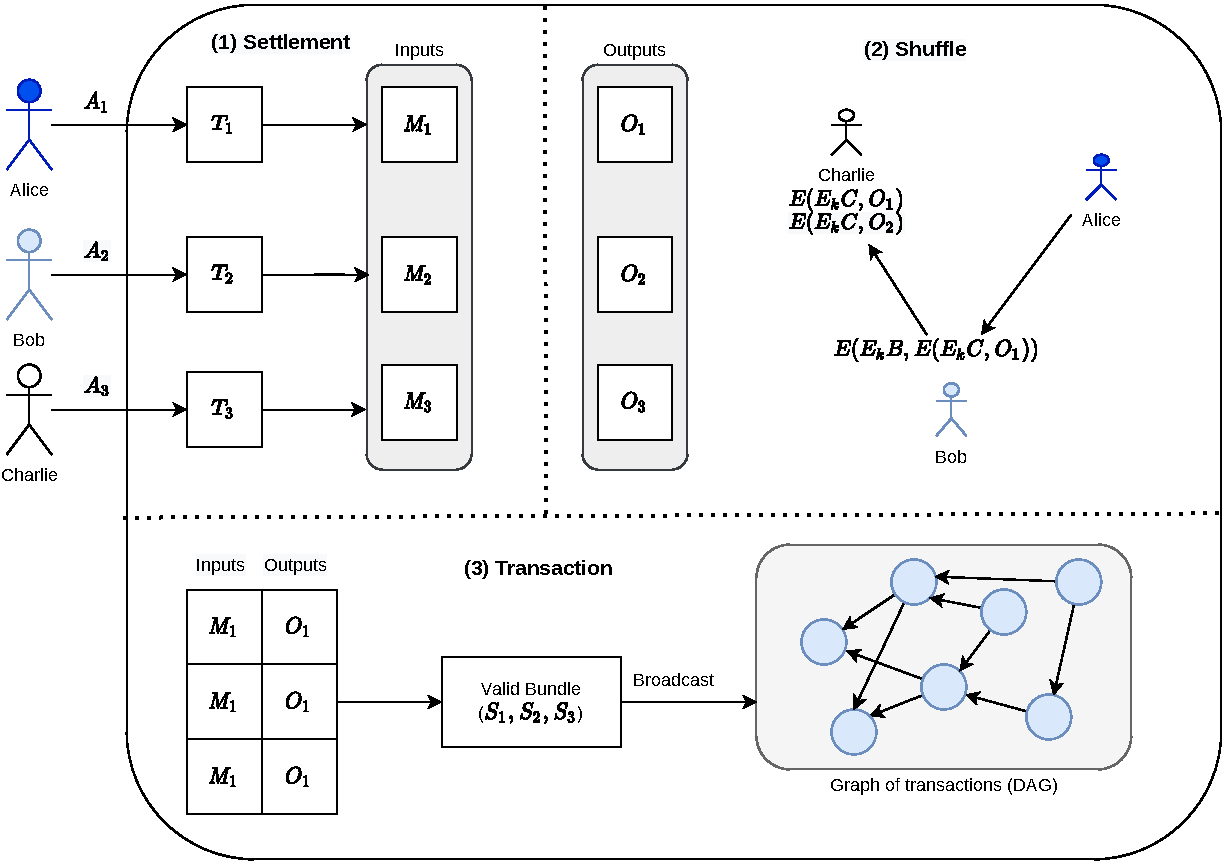
\includegraphics[width=\textwidth]{Images/mixing_iota.pdf}
  \caption{Three phases of decentralized mixing (settlement, shuffle, transaction) on the IOTA network with three peers \cite{Sarfraz2019}.}
  \label{F_mixing_iota}
  \end{figure*}
  
% \section{Performance optimization}
% \label{S_performance_optimization}

%   The proposed framework is designed to answer the performance, security and privacy needs of the Internet of Things. To ensure the system is consistent with the performance requirements, we assess the performance of the proposed framework in this section. In IOTA 2.0 \cite{Popov2020}, IOTA is decentralized and has a high throughput, low latency, high scalability and low storage overhead due to pruning.
%   However, the introduction of the UCS, IOTA Access and the mixing service likely introduces computation and network overheads, requiring further testing.
  
%   The evaluation of IOTA's network metrics, such as scalability and throughput is not addressed by this evaluation. This section aims at demonstrating the framework is viable even though it relies upon numerous technologies, and is evaluated in terms of:
%   \begin{itemize}
%       \item \emph{Quality of service}: the entire chain of events leading to access is completed in a reasonable time frame;
%       \item \emph{Computational power}: the hardware requirements are reasonable as regards Internet of Things constraints.
%   \end{itemize}
  
%   Regarding the Quality of Service, the focus is given to determining the time required for a user to be granted access after its payment. Average, minimum and maximum times will be considered. Additionally, several hardware configurations are tested, to assess whether the UCS can be deployed on resource-constrained devices.
   
%   \subsection{Configuration}
%   \label{ss_configuration}
  
%   \textbf{Configuration of the IOTA node.}
%   To reduce computation and network overheads introduced by the usage control system, several optimizations are set up: the usage control system deploys an IOTA node to integrate the IOTA network. This integration provides several benefits. The UCS can prioritize its transactions and perform local analysis on its ledger without querying the other IOTA nodes. Secondly, the IOTA node is configured, by removing the possibility to compute proofs of work for other users and by using \emph{spammers} to speed up the network by validating tips (cf. Section \ref{S_iota_dlt}), in particular when the network is in a low load regime.
%    Spammers are useful for testing as well, as the results are different whether the tests are conducted in a low load or high load regime.
%   The principles of integration, as well as its benefits, are fully detailed in the dedicated Section \ref{S_integration_usage_control_with_dlt}. 
%   As IOTA transaction throughput increases with the number of users, i.e. when many users push new transactions, it is relevant to use spammers that create zero-value transactions\footnote{zero-value transaction do not transfer iotas and the transaction corresponding amount is zero, hence their name} and validate two pending transactions from other users in the process. Spammers are implemented to ensure transactions do not take too long to be validated during low load regime.
%   Small devices with very poor computation capacities or with energy constraints can delegate their proof of work to a node. Our node is configured to refuse delegations to focus on usage control.
  
%   \textbf{Methodology and network configurations.}
%     We measure the time needed for a transaction to be validated and pushed to the network, and the time to fetch the transaction from an IOTA node. These operations correspond respectively to the calls \texttt{buildTransaction}, \texttt{push} and \texttt{checkTransaction} in the sequence diagram of Figure \ref{F_sequence_ifip}. 
%     Tests are conducted in three different configurations: (1) the IOTA remote node which is a resource-constrained node, to help understand the behavior of the solution in a fully constrained IoT environment, (2) the IOTA remote node which is no longer resource constrained to measure the gain from lifting the resource limitation, and (3) a local node which supports both the UCS and IOTA node, as illustrated in Figure \ref{F_framework_integration}.
%     For each test, one thousand samples ($N=1000$) are used. The resulting experimental measurements are summarized in Table~\ref{tab:metric}.

%     \textbf{Note on reproducibility.} The tests provided in this section are performed on the IOTA public test network. This is troublesome 
%     for reproducibility reasons (cf. Section \ref{ss_testbed}), but these tests have the following benefits:
%     \begin{itemize}
%       \item it is a first evaluation on a large-scale network to show that integration is a relevant process for performance. \cul{Addressing the challenges of large-scale networks is one of the purposes of this thesis work, justifying an evaluation on an appropriate network} (cf. Section \ref{S_assumptions}) ;
%       \item it enables estimating the outcomes of integration on a public network with a subsequent high number of nodes, rather than on a test network
%       with fewer nodes.
%     \end{itemize}

%     As a consequence, these tests are still considered in this chapter, not to demonstrate the validity of integration, but 
%     for informative purposes. Testing to demonstrate the validity of the integration process is provided in 
%     the dedicated section (Section \ref{S_performance_evaluation}) of Chapter \ref{C_integration}. 
%  \begin{figure*}[t]
%   \centering
%    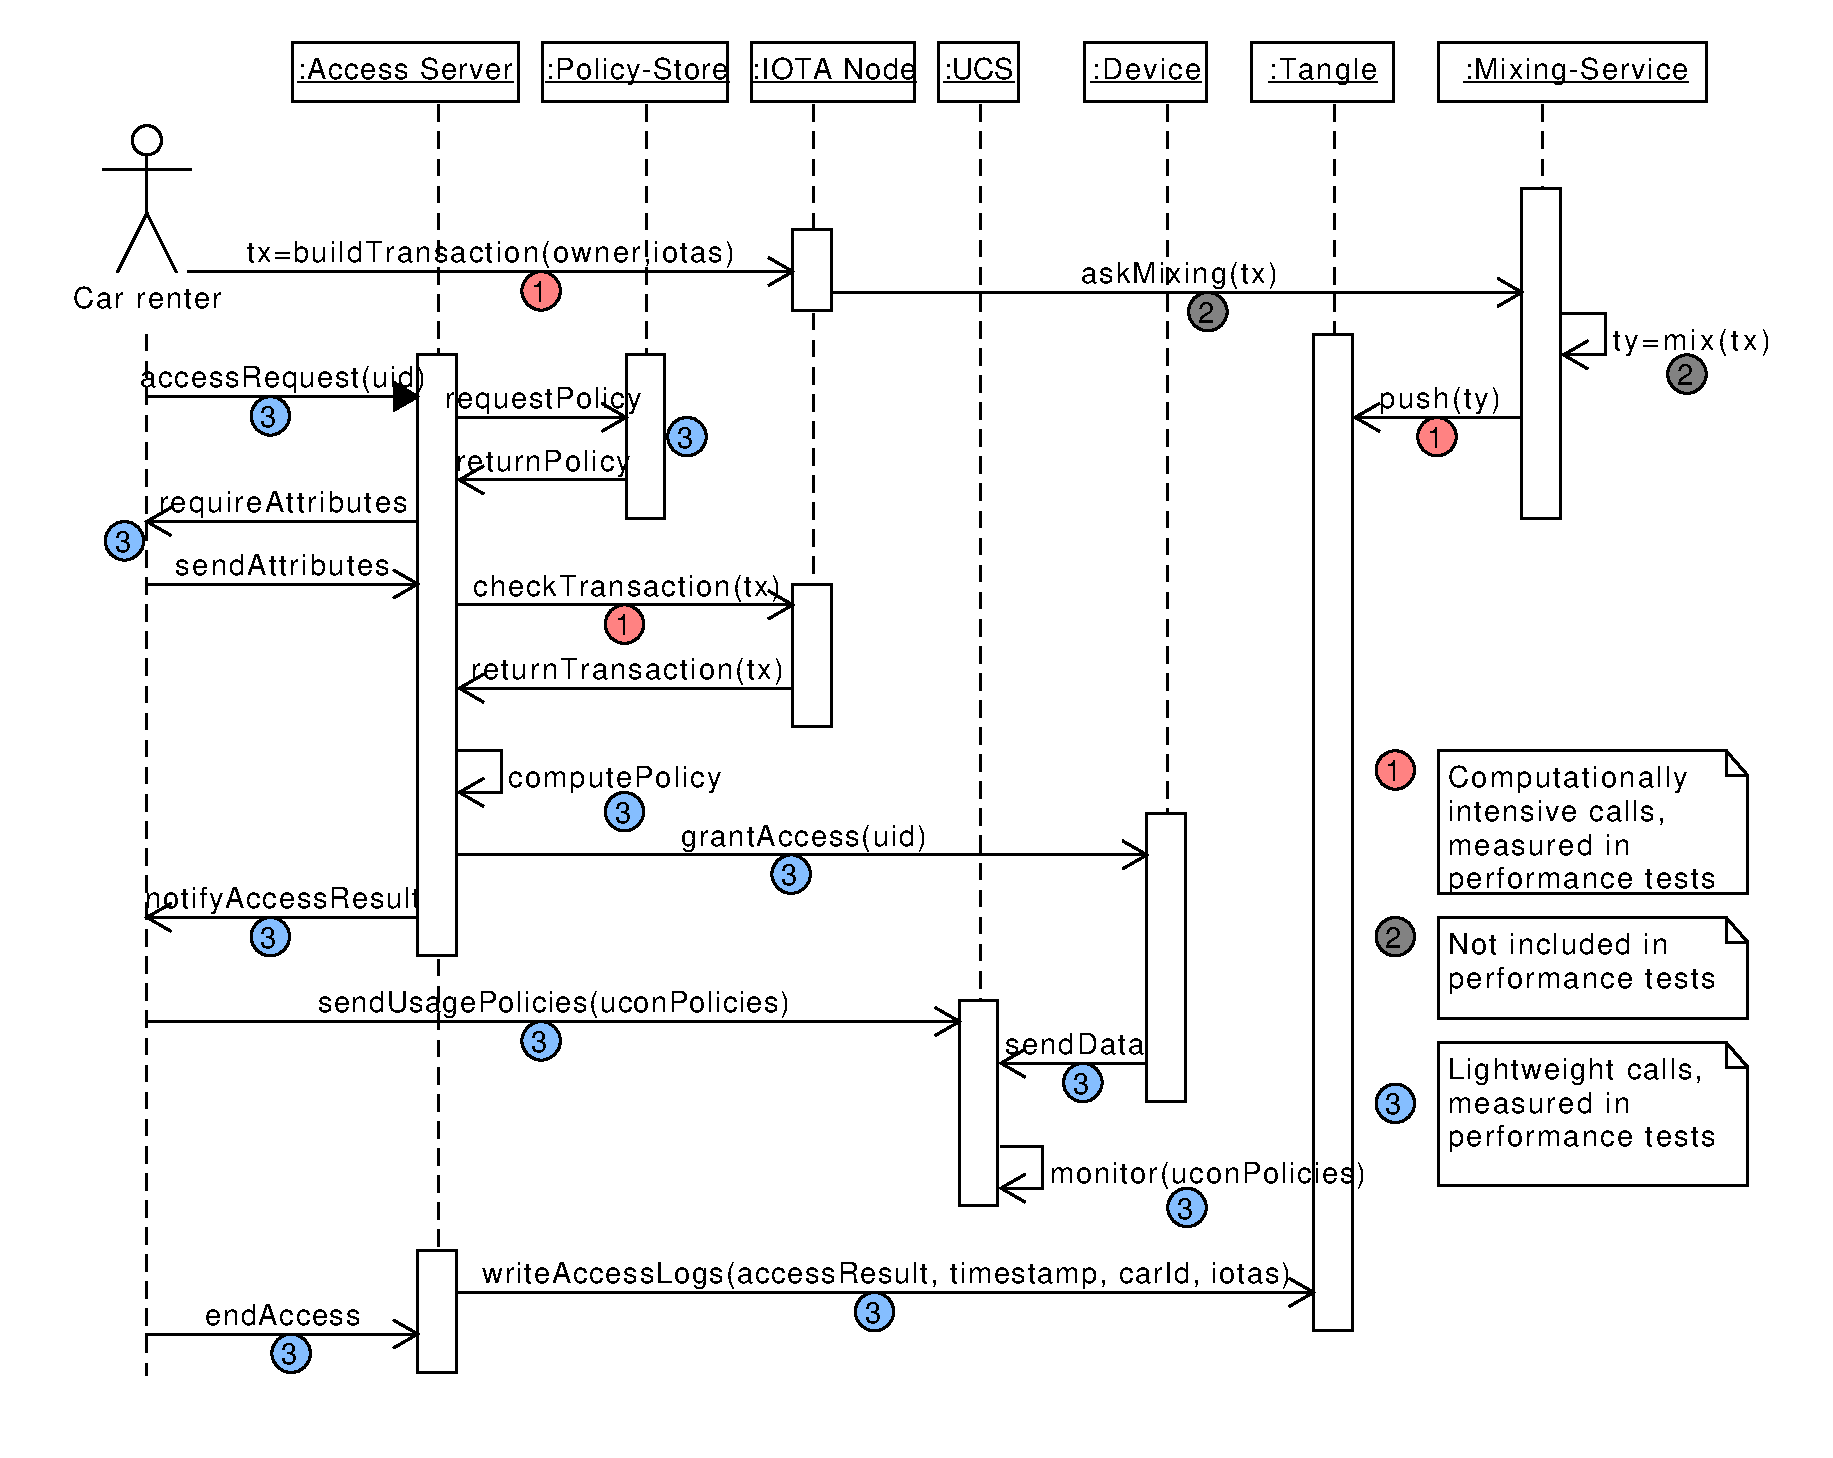
\includegraphics[width=\textwidth]{Images/sequence_ifip.pdf}
%   \caption{Workflow of a data access request using IOTA, IOTA Access and the mixing service.}
%   \label{F_sequence_ifip}
%   \end{figure*}

% \subsection{Evaluation results.}
%   \textbf{Resource-constrained remote testing.}
%     To demonstrate the possibility of a usage control system interacting with IOTA on resource-constrained devices, the performance tests are first conducted on a virtual machine with 4096MB of RAM and an Intel Core i5-10210U CPU @ 1.60GHz (1 core). The number of transactions per second \emph{on the test network} was oscillating between 3 TPS and 11 TPS on the test network, up to 16 with the spammer. The delegated proof of work is removed as part of the optimizations.
%     Pushing a transaction on a remote resource-constrained node (RCN) takes on average $\overline{t}_{push,rcn}= 5271ms$. Additionally, the usage control system takes an average $\overline{t}_{fetch,rcn}=45ms$ to fetch the transaction result from the remote node, accounting for a total $\overline{t}_{rcn}=5316ms$ on average as arithmetic mean is linear.
%     The time needed to create and push a transaction can tremendously vary, from a minimum $m_{rcn}=364ms$ to a maximum $M_{rcn}=26851ms$, which is reflected by a standard deviation of $\sigma_{rcn}=4629ms$. This difference is mostly due to the synchronization between peer nodes, which increases the transaction time significantly when the node is lagging or one of the peers disconnects. The confidence interval is $I_{rcn}=\overline{t}_{rcn}\pm1.96\frac{\sigma_{rcn}}{\sqrt{N}}=5316\pm287ms$.

%     The results show that the solution can be deployed on a machine with low computation capacities. However, with delays of up to 26 seconds to create, validate and push a transaction to the network, this can be unsatisfying in some use cases, e.g.  accessing a vehicle or 
%     opening a door lock.

% \textbf{Resource-unconstrained remote testing.}
% The IOTA remote node is now run on a computer with more computing power, with an Intel Core i5-10210U CPU @ 1.60GHz (4 cores) and 8192MB of RAM supporting the optimizations. This corresponds to the high-end Raspberry Pi 4 Model B specifications\footnote{https://www.raspberrypi.com/products/raspberry-pi-4-model-b/specifications/}.

% Pushing a transaction on a remote node (RN) with more computing capacity takes on average $\overline{t}_{push,rn}= 1867ms$. Additionally, the usage control system takes on average $\overline{t}_{fetch,rn}=45ms$ to fetch the transaction result from the remote node, accounting for a total $\overline{t}_{rn}=1912ms$ on average.
% The time needed to create and push a transaction is still very variable but spreads out less, from a minimum of $m_{rn}=363ms$ to a maximum of $M_{rn}=12209ms$, with a standard deviation of $\sigma_{rn}=1499ms$. The samples express a significant impact of the UCS computation power when creating and pushing transactions to a node. The confidence interval is $I_{rn}=\overline{t}_{rn}\pm1.96\frac{\sigma_{rn}}{\sqrt{N}}=1912\pm93ms$.

% The tests are also conducted using a much more powerful device, with 32GB RAM Memory and an Intel Core i5-1021UCPU @ 1.60GHz (8 cores). The purpose is to see if there is a limit in speed improvement as the UCS computation power increases. The results are very similar to the 8GB RAM setup, in the same confidence interval. 

% \textbf{Local testing.}
% The IOTA node is deployed on the local node (LN) running the UCS, as illustrated in Figure \ref{F_framework_integration}. The network connection, expressing the capacity of the local node to quickly get updates from other nodes, provides 98 Mbps in downlink and 77 Mbps in uplink. The node and the UCS run on the same device with 8192MB of RAM Memory and with the Intel Core i5-10210U CPU @ 1.60GHz (4 cores).
% The optimizations are also enabled. 
% The average time for a node to validate a transaction drops from $\overline{t}_{rn}=1912ms$ to an average $\overline{t}_{ln}=1579ms$. The minimum transaction time on a local node dropped from $m_{rn}=363ms$ to $m_{ln}=10ms$, while the maximum changed from $M_{rn}=12209$ to $M_{ln}=9830s$. The standard deviation is $\sigma_{ln}=1544ms$. The confidence interval is $I_{ln}=\overline{t}_{ln}\pm1.96\frac{\sigma_{ln}}{\sqrt{N}}=1579\pm96ms$.

% \begin{figure*}[t] 
%   \centering
%    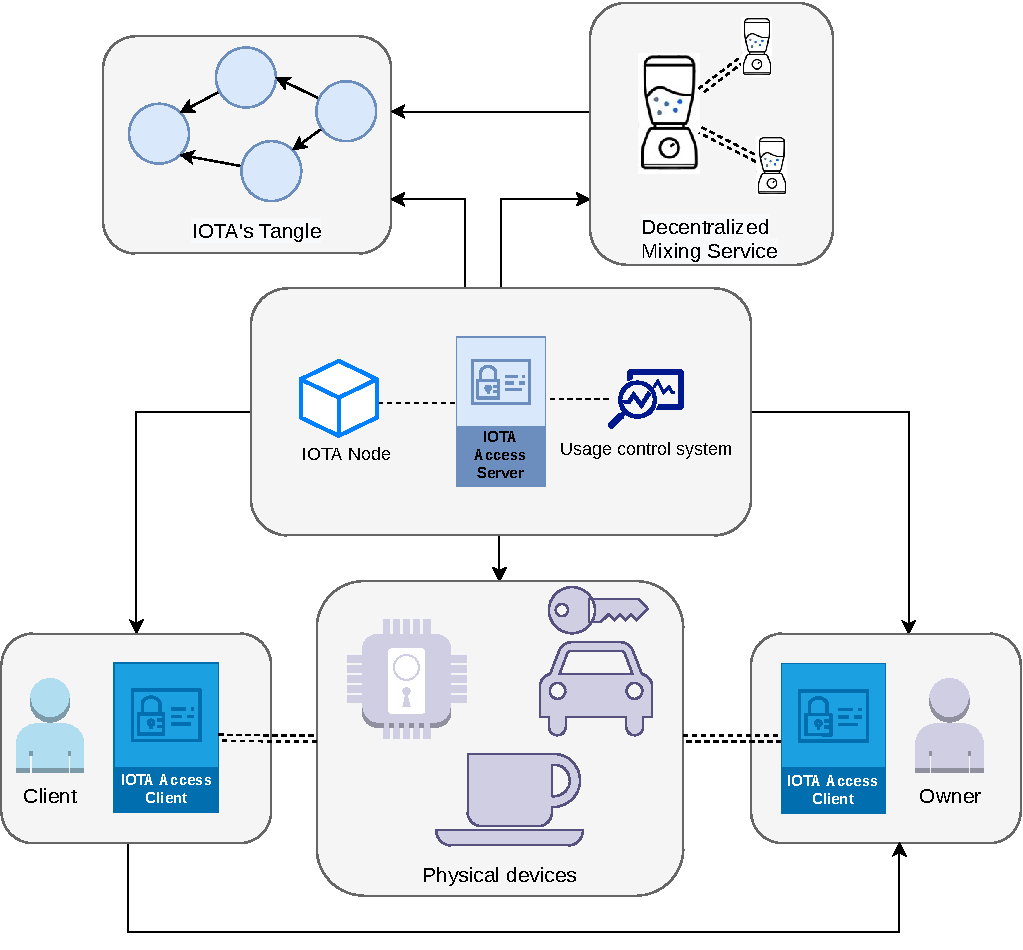
\includegraphics[width=0.68\textwidth]{Images/framework_IFIP_integration.pdf}
%   \caption{IOTA node deployment for optimization}
%   \label{F_framework_integration}
%   \end{figure*}
% % \subsubsection{Optimised local testing.}
% % The performance tests have been performed again with a local and optimised node (LO), on the same device as the UCS: first, the use of a spammer pushing four zero-value transactions per second. Secondly, the removal of delegated Proof of Work by our node. The average time for a node to validate a transaction further dropped from $\overline{t}_{ln}=1579ms$ to an average $\overline{t}_{lo}=XXXms$ on the local node. The minimum remained the same, $m_{lo}=10ms$ while the maximum further dropped from $M_{rn}=9830$ to $M_{lo}=XXXs$. The standard deviation is $\sigma_{lo}=XXXms$. The confidence interval is $I_{lo}=\overline{t}_{lo}\pm1.96\frac{\sigma_{lo}}{\sqrt{N}}=XXX\p

% As a result, using a local node has the following outcome:

% \begin{enumerate}
%     \item a 17.5\% decrease on the average transaction time;
%     \item transactions can be processed very quickly, taking a minimum of 10ms instead of a minimum $363ms$;
%     \item the maximum time only drops from $12209ms$ to $9830ms$, which remains convenient for real-life applications;
%     \item almost half (48\%) of the transactions are processed within a second, compared to 34.5\% for transactions using a remote node.
% \end{enumerate}

% \textbf{Additional calls.}
% While the performance tests are conducted on the three computationally intensive calls, the other category called \emph{lightweight calls} (cf. Figure \ref{F_sequence_ifip}) has also been measured. 
% The calls \texttt{accessRequest}, \texttt{requestPolicy}, \texttt{requireAttributes}, their corresponding return values \texttt{notifyAccessResult}, \texttt{sendAttributes}, \texttt{returnPolicy}
%  as well as \texttt{grantAccess} and \texttt{endAccess} consist in messages exchanged between the actors. They are strongly correlated to the time needed to communicate between the car renters, the access server, and the policy store. 
%  These calls took under 1ms to be achieved in our setup since they were all running locally on the same device. 
%  These three entities can be considered as close (in space) and the time for all these calls is negligible compared to the \texttt{buildTransaction}, \texttt{push} and \texttt{checkTransaction} calls.

% The remaining calls have different behavior. \texttt{computePolicy} is composed of several boolean operations, taking a negligible time. \texttt{sendUsagePolicies} and \texttt{sendGPSData} are operations
% that are continuously repeated until the access is terminated using the \texttt{endAccess} call or if \texttt{monitor} detects a violation of the policy. The time needed to \texttt{monitor} the access according to a given policy was measured and takes an average $\overline{p}=5ms$ for a simple policy made of three rules. 
% Finally, the call \texttt{writeAccessLogs} is very similar to \texttt{buildTransaction} as a message on IOTA is built as a zero-value transaction. However, it does not require checking balances and the construction of the transaction is simpler. A log takes an average $\overline{l}_{lo}=473ms$ to be built and pushed to 
% the network, on a local node using 1000 samples. Besides, the call \texttt{writeAccessLogs} does not impact the Quality of Service of the users as it is
% performed after the access is terminated.

% In conclusion, the experiments have shown that the framework fulfills the performance requirements, regarding the quality of service and the computational power (cf. Section \ref{S_performance_optimization}).  
% The time needed to validate the access to a user requiring it is acceptable, and resource-constrained devices can run a usage control system and interact with an IOTA node. 
% The IOTA node itself can run on a machine corresponding to Raspberry Pi Model B, as we did in the local testing section.  

%     \begin{table}[h]
%       \resizebox{\textwidth}{!}{%
%         \begin{tabular}{|c|c|c|c|c|}
%           \hline
%           \textbf{Test category} & \textbf{Min} & \textbf{Max} & \textbf{Average} & \textbf{Standard deviation $\sigma$} \\
%           \hline
%           Remote (constrained) & 364ms & 26851ms & 5316ms & 4629ms \\
%           Remote (unconstrained) & 363ms & 12209ms & 1912ms & 1499ms \\
%           Local & 10ms & 9830ms & 1579ms & 1544ms \\
%           \hline
%         \end{tabular}}
%         \caption{Performance measurements for different test configurations}
%         \label{tab:metric}
%       \end{table}    

\section{Security and privacy evaluation}
\label{S_security_and_privacy_evaluation}

As part of the research \hyperref[obj:56]{\emph{Objective 5}} (cf. Section \ref{S_problem_statement})
, this section analyzes the privacy and security risks in the system. To better identify the privacy and security threats and how they are mitigated by the proposed framework, we first introduce a car sharing illustrative scenario.

\subsection{Car sharing system illustrative scenario}
\label{ss_illustrative_scenario}


\emph{Car sharing} is a model of car rental where people rent cars for a short period. They differ from classic rental models in that the owners of the cars are individuals instead of an agency.
The context is dynamic as many users may enter or exit the car club during the day. For the users to interact with the system, a mobile application is used for registration and requiring access to the cars.

For security purposes, car owners have the right to monitor their cars and collect their real-time location. However, the location of the car also produces data about the car renters which are sent to the car owners. Car owners use a mobile phone application to define the access policy for their cars. Similarly, car renters define usage control policies using the same application. Car renters use public distributed ledger technology to make decentralized and transparent transactions. Car renters as well as car owners have one or several addresses on the IOTA network, to either send or receive transactions.


\subsection{System agents} The agents of the car renting system can be summarized as follows:

\begin{itemize}
    \item the car owners put their vehicles on the renting market;
    \item the car renters pay for renting the vehicles;
    \item the cars themselves send data to the owners such as location, and whose access is monitored;
    \item the Access Server (AS) is responsible for managing the access to the cars;
    \item the Usage Control System (UCS) monitors the data generated by other agents;
    \item the mixing server obfuscates the transactions to preserve privacy.
\end{itemize}

 Both the Access Server and the Usage Control System control access, respectively to a physical object - the car - and to the data. The UCS also monitors the information flow, blocking data dissemination to forbidden actors.

%  \rul{The next security and privacy threat analyses, in the context of the scenario, focus on the threats associated with the geolocation data of the car renter. As a consequence, the security analysis focuses on the usage control system as the main security component accountable for the privacy of the car renter. Note that apart from geolocation data, other kinds of data are privacy-sensitive and can be used to carry out inference attacks, such as the habits of car renters and car owners. Besides, the threat analysis could have been centered on car owners or on the decentralized mixing service, which are also privacy-sensitive. Yet, the choice to focus on car renters is motivated by the fact that the mitigations put in place can be extended to other privacy-sensitive data. Therefore, enumerating all possible threats in the system does not help to demonstrate the relevance of the framework and is a complex process.}
\subsection{Security and privacy threat model}
\label{ss_priv_threats}

\textbf{Privacy threat model.}
Depending on the data the attackers are obtaining, and using the LINDDUN threat evaluation framework \cite{Wuyts2015} (cf. Section \ref{ss_privacy_threat_modeling}), we discuss the threat analysis for our proposed scenario hereafter. 
\begin{itemize}
    \item \emph{linkability}(L): an attacker can link the car renter and the car owner, respectively the sender and the receiver of a transaction, thus simplifying re-identification and inference; 
    \item \emph{identification}(I): the attacker can link 
    the pseudonym to the real identity of the car renters or the car owners, breaking anonymity;
    \item \emph{Non-repudiation and repudiation}(N): With repudiation, an attacker can exfiltrate information and deny it did. Note that this threat is actually \emph{a security goal} in our system, contrary to other threats. Conversely, non-repudiation can be a threat to legitimate users if an attacker can prove that a user has done some sensitive actions e.g., an illicit transaction~\cite{Wuyts2015}. In our scenario, non-repudiation is not considered a threat, but repudiation is;
    \item \emph{disclosure of information}(D): an attacker can access data about a user without having the proper access rights. Inference attacks can be included in this category and are defined as "attacks where the attacker has used existing knowledge to aid the attack”~\cite{Henriksen2016}. An inference attack occurs when an attacker can infer information from apparently harmless information. For example, in our scenario, an attacker could infer working hours by gathering transactions timestamps;
    \item \emph{unawareness}(U): unawareness occurs if car renters are not aware of the collection, processing, sharing and storage of their geolocation data;
\end{itemize}

Detectability(D) is not considered a threat as data is publicly registered on the ledger. Both the existence and the content of the data are already known to the attackers. Rather than preventing detectability, the focus is given to preventing its most important aftermath, inference attacks~\cite{Wuyts2015}.
Non-compliance(N) is considered an orthogonal issue since the regulations are country-dependent. However, distributed ledgers may have several compliance issues, such as their immutability which contravenes articles 16, 17 and 18 of the GDPR about the right to data deletion and modification~\cite{EUdataregulations2018}. Finding technical solutions to compliance issues is an active field of research~\cite{Haque2021}.

\textbf{Security threat model}
\label{ss_sec_threats}
Considering the agents defined in the car renting system, the threat model distinguishes \emph{four attacker types}:
\begin{enumerate}
    \item the single car owner, who has legitimate access to some sensitive data of the car renters;
    \item several car owners colluding to gather bigger sets of data;
    \item the mixing server that may secretly keep the links between car renters and car owners that it is supposed to remove. It can use this information to carry out re-identification attacks; 
    \item external attackers who wish to disable the UCS to help car owners disseminate data to other agents.
\end{enumerate}

The car owners are considered \emph{honest-but-curious}. They will respect the system rules by granting access to their cars upon receiving payments but will snoop on the data of the users requesting their services. Honest-but-curious attackers are assumed to rely on transactional content only to re-identify users, rather than network-level information, e.g. IP addresses. External attackers are conversely \emph{malicious} and actively try to neutralize the UCS to enable car owners to disseminate their data.

Concurrently, there are \emph{security risks} because a single agent of the system - namely the UCS - is responsible for data protection. The UCS itself is considered as \emph{trusted}. External attackers can however be interested in neutralizing the UCS to enable the collusion of car owners. Similarly to the privacy threat analysis using LINDDUN, we use the STRIDE security threat modeling \cite{Howard2006} to identify the security threats for the usage control system:
\begin{itemize}
    \item \emph{Spoofing}(S): an external attacker could masquerade as a legitimate user to be granted access to unauthorized data, or as the control system to collect the car renters' data;
    \item \emph{Tampering}(T): an external attacker could modify either the data or the infrastructure of the usage control system. Besides, an attacker could try to modify the binaries of the usage control system to make it ineffective~\cite{Kelbert2018};
    \item \emph{Denial of service}(D): the external attacker can temporarily disable the UCS, threatening the availability of the system and disabling the usage control mechanisms.
\end{itemize}

The Repudiation(R) and Information disclosure(I) risks are already tackled by the LINDDUN privacy threat model and are excluded from the security threat modeling. Finally, an external attacker can conduct an Elevation of privilege(E) by leveraging vulnerabilities as illustrated in~\cite{Babil2013} to bypass the UCS restrictions. These attacks are very diverse and implementation-dependent, therefore considered out of the scope of this thesis work.

\subsection{Privacy threats and mitigations.}
\label{ss_privacy_threats_and_mitigations} 

 Table~\ref{l_table1} describes for inference attacks each possible combination of attackers, the data types they have access to, where data is stored and an instance of a privacy leakage associated with this risk. Table~\ref{l_table2} describes other privacy threats and how they are mitigated.\rul{The focus is put on car renters as an example but the mitigations introduced can be applied to other privacy-sensitive data if: 1) the data dissemination is a privacy risk; 2) the data processing creates inference risks. Such data also include but are not limited to the car renter's driving habits or the car owner's renting habits.}

\begin{table}[h]
  \resizebox{\textwidth}{!}{%
    \begin{tabular}{|c|c|c|c|}
      \hline
      \textbf{Attacker type} & \textbf{Data type} & \textbf{Data storage} & \textbf{Example} \\
      \hline
      Honest-but-curious & Transaction & Tangle & Purpose of payment \\
      Car owner (alone) & Location & Owner's device & Renter's job \\
      Car owners (colluding) & Location & Owners' devices & Renter's job \\
      Ext. attacker \& car owners & Location & Owners' devices & Data sets on renters \\
    % Mixing service & Pseudonym &  Mixer memory & Linkage, identification & Identities of users\\ 
      \hline 
    \end{tabular}}
    \caption{Inference attacks according to the attackers' profile}
    \label{l_table1}
  \end{table}
  
Any user has access to the Tangle's transactions, which are public and contain privacy-sensitive timestamps, users' addresses and values, i.e. how many iotas are sent to a car owner. Any honest-but-curious attacker can attempt to use the blockchain transactions for inference attacks, e.g. use the number of tokens in the transactions to infer the purpose of the payment. The merge avoidance mechanism integrated into our framework reduces the risk of inference by splitting the transactions into several smaller ones, thus making it harder to guess the purpose of the transactions (cf. Section \ref{ss_obfuscation_coin_mixing_merge_avoidance}). \rul{For instance, it is harder to infer the benefits of the car owners as long as sub-addresses are not linked with one another, or to identify the purpose of the car renters transactions.}

Additionally, car owners may infer privacy-sensitive data from the car renters' location data. The location of the car renters may reveal their driving habits, their jobs, their religion or their hobbies.
Besides, colluding car owners can merge their data about a given user to increase the inference's quality or increase the number of users in their databases to improve their value.
If an external attacker successfully neutralizes the UCS, as reported in Section~\ref{ss_security_threats_and_mitigation}, car owners can freely share users' data and disseminate them to a shared database for processing. 

\begin{table}[h]
  \resizebox{\textwidth}{!}{%
    \begin{tabular}{|c|c|c|c|}
      \hline
      \textbf{Attacker type} & \textbf{Data type} & \textbf{Threat} & \textbf{Mitigation} \\
      \hline
      Honest-but-curious & Transaction & Linkability & Mixing \\
      Honest-but-curious & Transaction & Identification & No address reuse \\
      Curious Mixer & Addresses & Linkability & Mixer decentralization \\
      External attacker & Geolocation data & Disclosure & Usage and Data Flow Control \\
      Car owner & Renters' data & Repudiation & Data flow control, auditability \\
      Honest-but-curious & Renters' data & Unawareness & Usage control \\
      \hline
    \end{tabular}}
    \caption{Threats to privacy and their mitigation}
    \label{l_table2}
  \end{table}
Table \ref{l_table2} summarizes the privacy threats for the car renters excluding inference attacks, here above presented. By observing transactions, an honest-but-curious attacker may try to link the sender and the receiver. This risk is mitigated by the mixing server. Furthermore, when car renters use the same address multiple times for outward transactions, they are exposed to re-identification (cf.~section~\ref{ss_de_anonymisation}). We generate a new address in our framework for each outward transaction and forbid address reuse to mitigate this risk. Moreover, as the mixing service is decentralized (cf. Section \ref{ss_decentralized_mixing_iota}), a node involved in the mixing process can not make links between any input or output addresses. The information disclosure is prevented by the usage control system, as it monitors access to the data and prevents dissemination to unauthorized users. The repudiation threat is provided as the car owners are continuously monitored by the UCS. Finally, usage control provides a solution to unawareness as car renters have to explicitly specify how they want their data to be used. 

\subsection{Security threats and mitigation}
\label{ss_security_threats_and_mitigation}
The UCS is a critical agent for controlling data usage and data flows between the system agents. It is an attractive target, vulnerable to specific attacks which can be partially mitigated. The proposed countermeasures to the security threats established using the STRIDE model (cf. section \ref{ss_sec_threats}) are:
\begin{itemize}
    \item \emph{Spoofing}(S): legitimate users and the usage control system mutually authenticate, e.g., using SSH or TLS;
    \item \emph{Tampering}(T): the data processing is monitored by the UCS, excluding illegal modifications to the data. However, an attacker can modify the usage control system's binaries to make it ineffective~\cite{Kelbert2018}. This threat can be mitigated by digital signatures~\cite{Kelbert2018};
    \item \emph{Denial of service}(D): the modern denial of service attacks can be hard to mitigate, but decentralizing the UCS alleviates the risk, as well as mutual authentication of all the infrastructure components using certificates~\cite{Kelbert2018};
\end{itemize}

\rul{In addition to the security threats addressed by STRIDE, we complement the analysis with another critical physical security issue, which is the possibility to damage the car.}
 Car renters may damage the car and it is relevant to design a compensatory measure to make sure the car owners do not take disproportionate risks by getting involved in the network. Indeed, the framework provides a fair level of privacy and car renters are encouraged to run away without paying compensation for damaging the car. This is a strong deterrent to the car owners' involvement in the system.
As a solution, we introduce a stake that has to be locked by the car renter during a given amount of time in the form of a UCON pre-obligation. This principle is very similar to the proof of stake but is used to make access decisions rather than to achieve consensus. In proof of stake, smart contracts are needed to automatize both the rewards and the penalties, respectively for right or wrong behaviors. In our stake guarantee system, smart contracts are used to withdraw the deposit or conversely to give it back to the car renters once the access and the arbitration time are over. However, smart contracts are not yet fully implemented in IOTA, and can only be used in the test network~\cite{SC2021}. An alternative is to send the deposit to an address belonging to the usage control system as long as smart contracts are not available. Although less satisfying, this is a convenient workaround under the trusted UCS assumption.

\section{Conclusion}
\label{S_conclusion_ifip}

In this chapter, we detailed and evaluated a framework to address the requirements of privacy, security and
performance of the Internet of Things, while providing a basis for zero-fee micro-transactions (\hyperref[obj:1]{\emph{Objective 1}}). 
The basis of the framework is the IOTA DAG-based distributed ledger.
IOTA is complemented by privacy-preserving mechanisms: merge avoidance
and decentralized mixing. Finally, we added usage control so that users can monitor the usage of their data, 
and data providers sell the data generated by their devices according to pre-defined policies, including rules on transactions.

\cul{We conducted security and privacy evaluations as part of the \hyperref[obj:56]{\emph{Objective 5}} (cf. Section} \ref{S_problem_statement}) \cul{to highlight the security and privacy guarantees provided by the framework}.
The next chapter \ref{C_integration} introduces an integration method to further improve performance aspects. 
We analyze the necessary conditions to ensure integration is relevant, provide a methodology to integrate usage control 
before evaluating the outcome of the proposed integration.
 